% ==========================================
% Section 4: Unbalanced Distribution (Slides 13-16)
% ==========================================

% Slide 13: Unbalanced Distribution
\begin{frame}{توزیع نامتوازن کلاس‌ها}
\begin{columns}[c]
  \begin{column}{0.55\textwidth}
    \begin{itemize}
      \item \textbf{مثال: یادگیری مدلی برای تشخیص \lr{HIV}}
      \begin{itemize}
        \item با توجه به مجموعه‌ای از علائم بالینی
      \end{itemize}
      \vspace{0.15cm}
      \item \textbf{مجموعه داده:}
      \begin{itemize}
        \item پرونده بیمارانی که از نظر ابتلا به \lr{HIV} آزمایش شده‌اند
      \end{itemize}
      \vspace{0.15cm}
      \item \textbf{توزیع کلاس‌ها:}
      \begin{itemize}
        \item \lr{99.9\%} منفی (\lr{Negative})
        \item \lr{0.1\%} یا \lr{0.01\%} مثبت (\lr{Positive})
      \end{itemize}
      \vspace{0.15cm}
      \item \textbf{یادگیری درخت تصمیم:}
      \begin{itemize}
        \item یافتن هرگونه انشعاب با بهبود کیفیت معنادار بسیار دشوار خواهد بود.
        \item درخت تصمیم آموخته‌شده تنها یک خروجی همواره «منفی» پیش‌بینی می‌کند.
      \end{itemize}
    \end{itemize}
  \end{column}
  \begin{column}{0.43\textwidth}
    \centering
    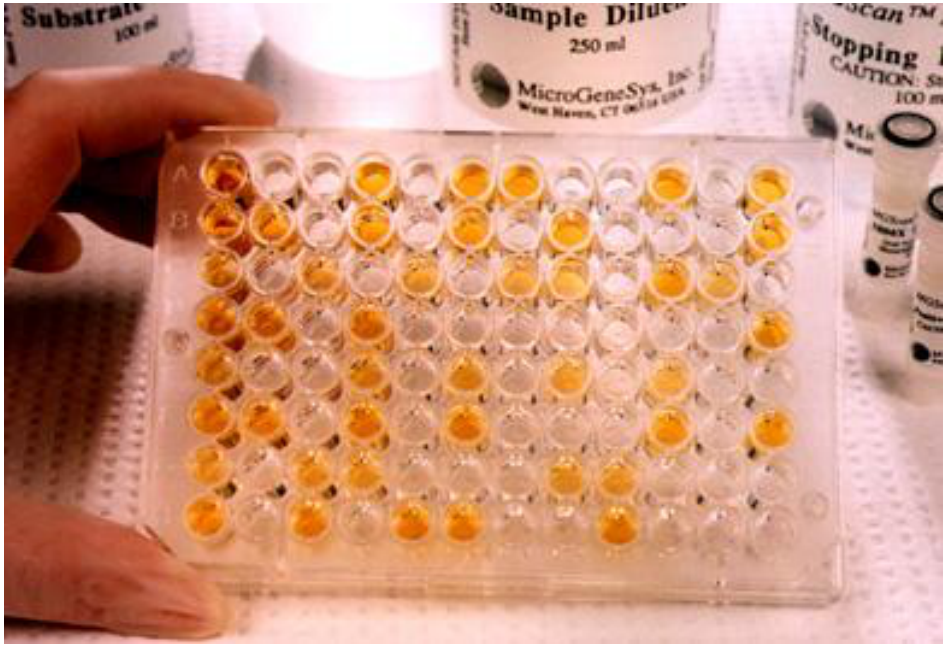
\includegraphics[width=\textwidth]{images/page_13_img_1.png}
  \end{column}
\end{columns}
\end{frame}

% Slide 14: Resampling Unbalanced Data
\begin{frame}{بازنمونه‌گیری داده‌های نامتوازن}
\begin{itemize}
  \item \textbf{دو هدف متناقض:}
  \begin{itemize}
    \item استفاده از حداکثر داده‌های آموزشی ممکن (\lr{Use as much training data as possible})
    \item استفاده از حداکثر تنوع در داده‌های آموزشی (\lr{Use as diverse training data as possible})
  \end{itemize}
  \vspace{0.4cm}
  \item \textbf{استراتژی‌های بازنمونه‌گیری (\lr{Resampling}):}
  \begin{itemize}
    \item \textbf{زیرنمونه‌گیری از کلاس اکثریت (\lr{Downsampling}):}
    \begin{itemize}
      \item در تضاد با هدف اول (داده‌های زیادی دور ریخته می‌شود)
    \end{itemize}
    \vspace{0.2cm}
    \item \textbf{بیش‌نمونه‌گیری از کلاس اقلیت (\lr{Upsampling}):}
    \begin{itemize}
      \item در تضاد با هدف دوم (تنوع جدیدی اضافه نمی‌شود)
    \end{itemize}
  \end{itemize}
\end{itemize}
\end{frame}

% Slide 15: Resampling Extreme Example
\begin{frame}{بررسی یک سناریوی حدی از عدم توازن}
\begin{columns}[c]
  \begin{column}{0.55\textwidth}
    \begin{itemize}
      \item \textbf{یک مثال حدی را در نظر بگیرید:}
      \begin{itemize}
        \item \lr{1,000} نمونه از کلاس \lr{A}
        \item \lr{10} نمونه از کلاس \lr{B}
      \end{itemize}
      \vspace{0.2cm}
      \item \textbf{زیرنمونه‌گیری (\lr{Downsampling}):}
      \begin{itemize}
        \item \lr{990} نمونه را استفاده نمی‌کند و نادیده می‌گیرد.
      \end{itemize}
      \vspace{0.2cm}
      \item \textbf{بیش‌نمونه‌گیری (\lr{Upsampling}):}
      \begin{itemize}
        \item از هر نمونه کلاس \lr{B} تعداد \lr{100} کپی ایجاد می‌کند.
        \item طبقه‌بند تمایل پیدا می‌کند صرفاً این \lr{10} نمونه کلاس \lr{B} را حفظ کند!
      \end{itemize}
      \vspace{0.2cm}
      \item \textbf{کتابخانه پایتون:}
      \begin{itemize}
        \item \url{https://imbalanced-learn.org/}
      \end{itemize}
    \end{itemize}
  \end{column}
  \begin{column}{0.43\textwidth}
    \centering
    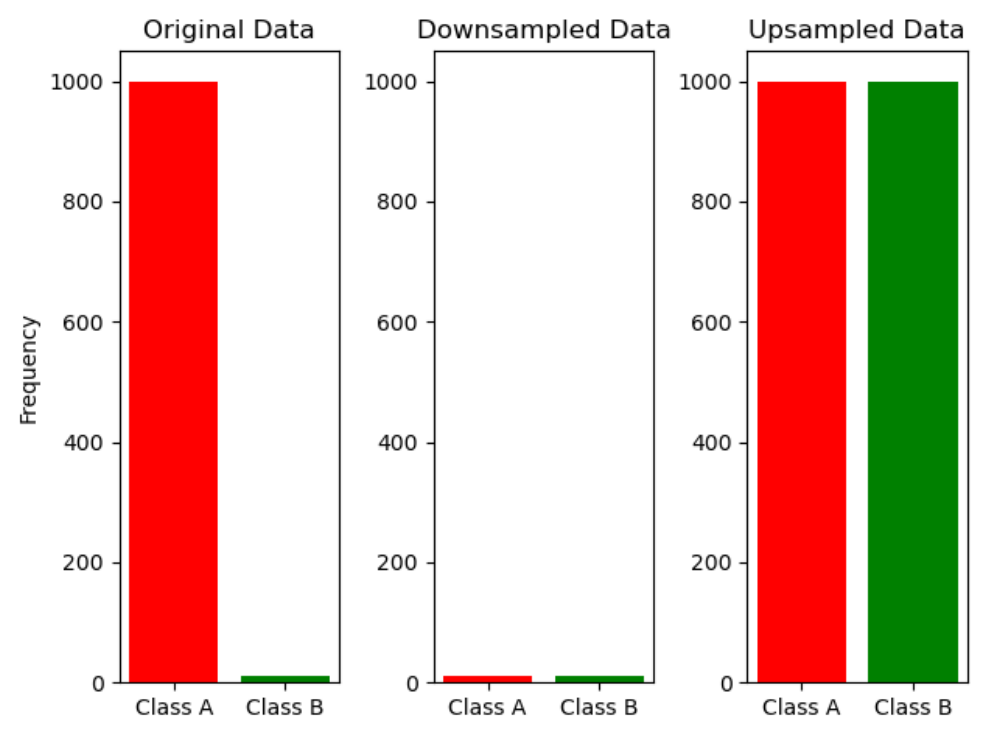
\includegraphics[width=\textwidth]{images/page_15_img_1.png}\\[8pt]
    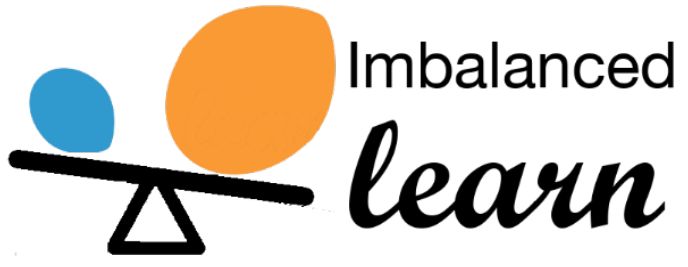
\includegraphics[width=0.75\textwidth]{images/page_15_img_2.png}
  \end{column}
\end{columns}
\end{frame}

% Slide 16: SMOTE
\begin{frame}{تکنیک بیش‌نمونه‌گیری اقلیت مصنوعی (\lr{SMOTE})}
\begin{columns}[c]
  \begin{column}{0.58\textwidth}
    \begin{itemize}
      \item \textbf{روش \lr{SMOTE} (تکنیک بیش‌نمونه‌گیری اقلیت مصنوعی)}
      \begin{itemize}
        \item ساخت نمونه‌های مصنوعی از کلاس اقلیت
      \end{itemize}
      \vspace{0.2cm}
      \item \textbf{مراحل الگوریتم برای نمونه مفروض $x$:}
      \begin{itemize}
        \item انتخاب یک همسایه $n$ در میان $k$ نزدیک‌ترین همسایه (درون همان کلاس) $x$
        \item ایجاد نمونه مصنوعی $s$:\\
        \vspace{0.1cm}
        به ازای هر ویژگی $a$:
        $$s.a \leftarrow x.a + \text{rand}(0,1) \times (n.a - x.a)$$
      \end{itemize}
    \end{itemize}
  \end{column}
  \begin{column}{0.40\textwidth}
    \centering
    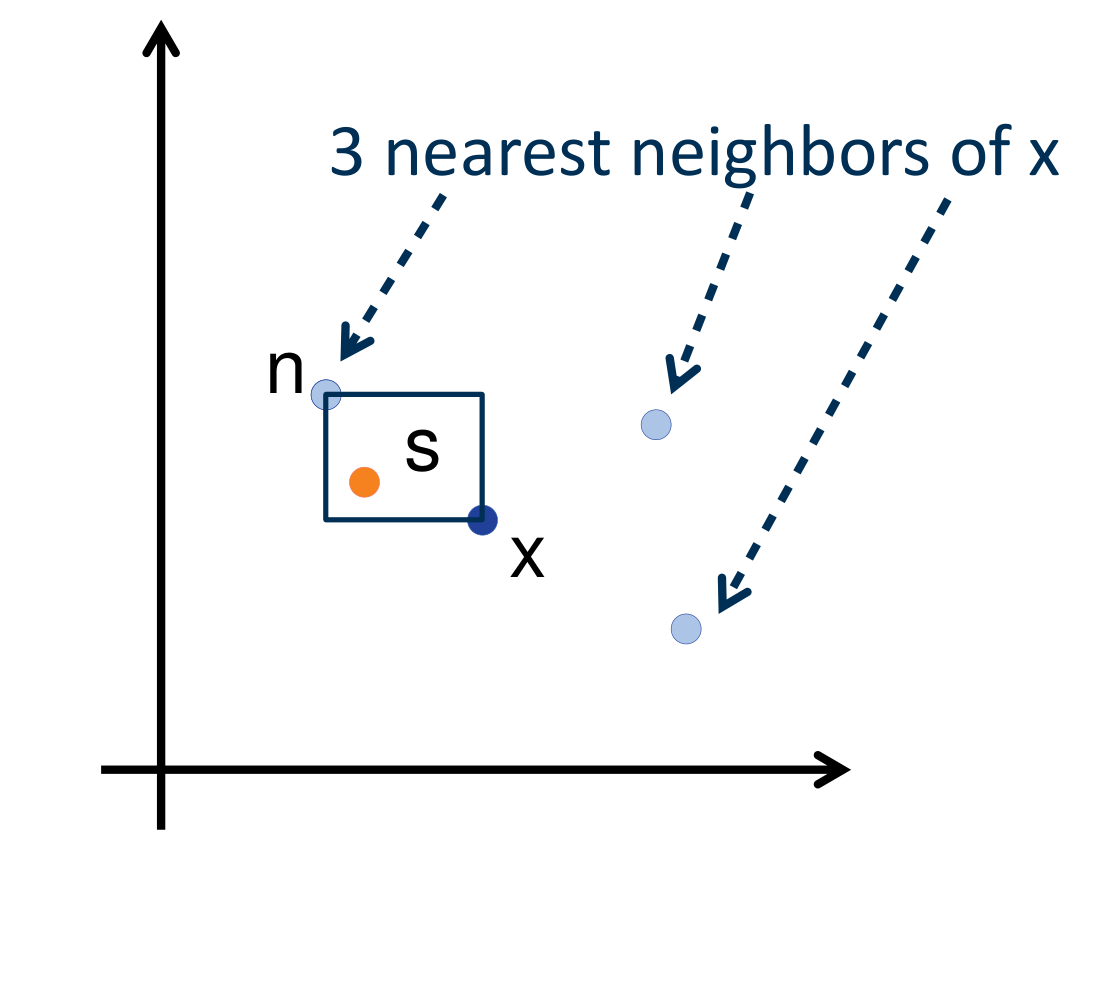
\includegraphics[width=\textwidth]{images/page_16_smote.png}
  \end{column}
\end{columns}
\vspace{0.2cm}
\flushright
{\fontsize{6.5}{8}\selectfont\color{subgray}مرجع اصلی: \lr{Chawla, Bowyer, Hall, Kegelmeyer (JAIR, 2002)}}
\end{frame}
